\section{De Bruijn Graphs}\label{sec:DBG}

The first concept to introduce in this section will be that of the De Bruijn Graph (DBG)~\cite{DeBruijnGraph}, which are used throughout much of bioinformatics.
However, first some notation must be presented.
A graph $G=\{V,E\}$ consists of a set of vertices $V=\{v_1,v_2,\ldots,v_n\}$ which are connected by a set of edges $E=\{e_1, e_2, \ldots, e_m\}$.
The terms nodes and vertex will be used interchangeably.
Each vertex $v_i$ has a label $label(v_i)$, a set of outgoing nodes $out_v(v_i)$ of size $\#out_v(v_i)$, a set of incoming nodes $in_v(v_i)$ of size $\#in_v(v_i)$, a set of outgoing edges $out_e(v_i)$, and a set of incoming edges $in_e(v_i)$, of sizes with the same notation as the vertices.
Then, $v_1$ has an outgoing edge to $v_2$ if there exists an edge $e$ such that $e=v_1 \rightarrow v_2$.
Each edge $e_i$ also has a label $label(e_i)$.

To construct the DBG, the dataset must be transformed.
Given a set of FASTA and FASTQ files, all the sequences must first be extracted individually, and then, using a sliding window method, extract all unique substrings of a set size $k$.
These substrings are called $k$-mers, historically introduced as \textit{k-tuples}~\cite{DeBruijnGraph}.
Formally, given a sequence $S=[c_0, c_1, \ldots, c_{C-1}]$ of size $C$, a set of sequences $\{ [c_0,c_1,\ldots,c_{k - 1}], [c_1, c_2,\ldots,c_{k}], \ldots , [c_{C-k}, c_{C-k+1}, \ldots, c_{C - 1}]\}$ is extracted.
Often, the reverse complements of these $k$-mers are also computed and added to the set of unique $k$-mers.
For this reason, the size of $k$ is usually taken to be an odd number, in order to avoid palindromes between the forward and backwards sequence which can cause problems for some analysis tasks~\cite{Palindromes}.
An example of a palindrome may be \textit{AGCGCT}, where the reverse complement of this sequence would be itself.

Now graph construction may commence.
Given a pair of $k$-mers with sequences $S_0=[a_0, a_1, \ldots, a_{k - 1}]$ and $S_1=[b_0, b_1, \ldots, b_{k - 1}]$, one must first create the nodes $v_0$ and $v_1$ for these $k$-mers and give them the labels $S_0$ and $S_1$ respectively.
Then if the $k-1$ suffix of $S_0$ is equal to the $k-1$ prefix of $S_1$, that is, $[a_1, a_2, \ldots, a_{k - 1}] = [b_0, b_1, \ldots, b_{k-2}]$, create an edge $v_0 \rightarrow v_1$.
The labels of the edges are the character that is added in order to get to the next $k$-mer, that is, the final character of the outgoing node $v_1$, which is $b_{k - 1}$.
This is done for all $k$-mers which share a $k+1$ suffix and prefix.
Figure~\ref{fig:FastaqToDbg} shows an example of the whole pipeline from the FASTA/FASTQ files to a DBG.\@

\begin{figure}[t]
  \centering
  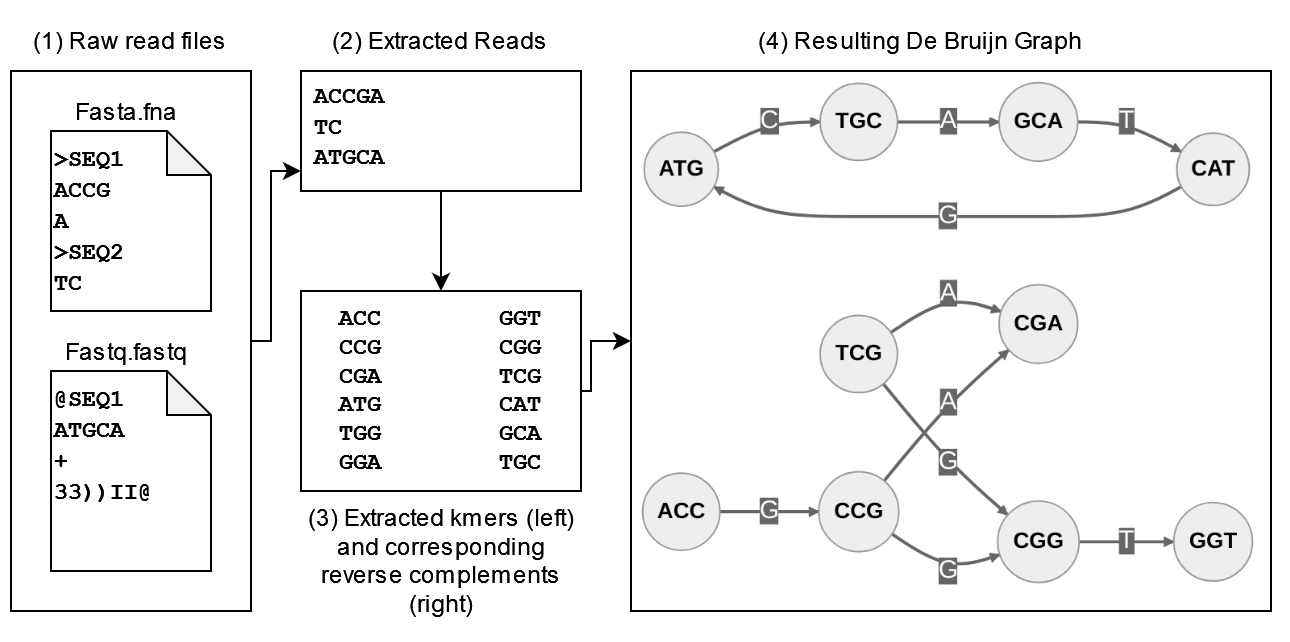
\includegraphics[width=\textwidth]{images/FastaqToDbg.png}
  \caption{The pipeline from FASTA/FASTQ files to the final DBG with $k = 3$.}\label{fig:FastaqToDbg}
\end{figure}

The DBG is a crucial part of many genome analysis tasks.
For example, it can be used to assemble a new genome by traversing it, and if there is a single Eulerian path for the entire graph, then it is known that this is the order in which reads must be assembled~\cite{DeBruijnGraph}.
An Eulerian path is a path that traverses all edges exactly once.
Note that this would not work for the graph in Figure~\ref{fig:FastaqToDbg}, but Figure~\ref{fig:EulerianPath} shows a good example of this.
That said, even this example may not be perfect, because the graph also consists of an unknown number of repeats.
Much work has been done to improve on assembly techniques of new genomes based on this method, especially tackling ambiguity issues when a single Eulerian path might not be possible, such as by giving more weight to certain nodes when they meet certain conditions~\cite{DeBruijnGraph, EulerianPath}.
Some readers may have already started thinking of ways to tackle the many potential challenges of such a problem~\cite{ModernAssembly}, however, this text will not be going into more detail about these assembly methods as they are not relevant to the rest of the contents.

\begin{figure}[t]
  \centering
  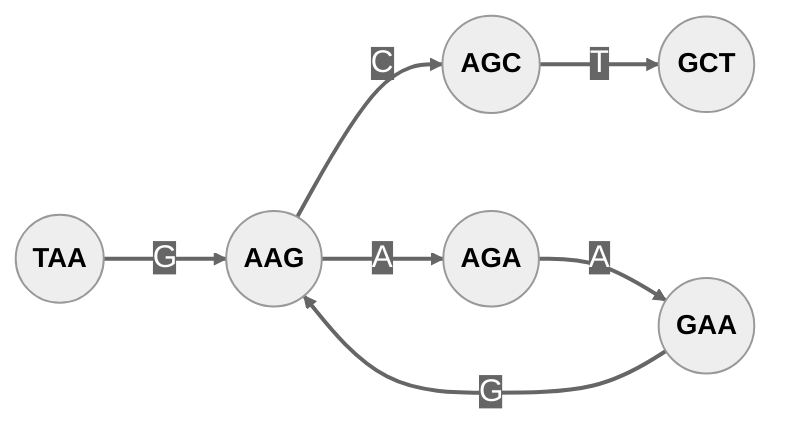
\includegraphics[width=0.6\textwidth]{images/EulerianPath.png}
  \caption{An example of a DBG with $k = 3$ where one can trace a perfect Eulerian path. This path is $TAAGAAGCT$.}\label{fig:EulerianPath}
\end{figure}

From Figure~\ref{fig:EulerianPath}, some properties of its graph can also be pointed out, relating to contigs and unitigs, the former of which was discussed in Section~\ref{sec:Biology}.
For example, the contigs which pass through the nodes $\mathit{TAA} \rightarrow \mathit{AAG} \rightarrow \mathit{AGC} \rightarrow \mathit{GCT}$ can be seen, and the other contig would be the path $\mathit{TAA} \rightarrow \mathit{AAG}$ and $\mathit{AGA} \rightarrow \mathit{GAA}$.
However, none of these are unitigs, because the paths to these contigs branch at the vertex \textit{AAG}.
In this example, one can find the unitig paths $\mathit{TAA}$, $\mathit{AGA} \rightarrow \mathit{GAA}$, $\mathit{AGC} \rightarrow \mathit{AGC}$.
Hence, a unitig is defined as a maximal path with no branching nodes, that is, for all $v_i$ in the path of size $n$, $out_v(v_i) = 1, i = 0,\ldots,n - 2$ and $in_v(v_j) = 1, i = 1,\ldots,n - 1$~\cite{Themisto}.
For the purposes of this text, in Section~\ref{sec:Pseudoalignment}, contigs will not be of use, but unitigs are an important concept and they will further expanded on.

For the SBWT~\cite{SBWT}, which is discussed in Section~\ref{sec:SBWT}, and thus also for this thesis, each node must have at least one incoming node.
To solve this, the nodes without an incoming node, that is, all vertices where $\#in(v_i) = 0$, are taken, and a new node which has the first character a \textit{\$} symbol is added, and the rest of the characters are the first $(k-1)$ characters of the sequence corresponding to the original node.
As an example of these nodes, given a node without any incoming edges corresponding to the $k$-mer $AAT$, one would add a new node $\$AA$.
Recursively, another node is added in the same manner to the new node.
The base case is when the final node which has $k$ $\$$-symbols is added.
Therefore, in the case of the previous example, the nodes $\$\$A$ and $\$\$\$$ are also added.

This means that the alphabet size is now 5: \textit{ACGT} and \textit{\$}.
However, make an important mental note that the nodes never point to another node whose corresponding sequence ends with a $\$$-symbol, that is, no edge will ever contain a $\$$-symbol as a label.
The only sequence which ends with a $\$$-symbol is $\$\$\$$, and this is the only node that does not have any incoming edges.
Thus, it will be seen that there is no need to worry about the expanded alphabet size later on, due to this property.
The altered results from Figure~\ref{fig:FastaqToDbg} are found in Figure~\ref{fig:FastaqToDbgWithDollars}.

\begin{figure}[t]
  \centering
  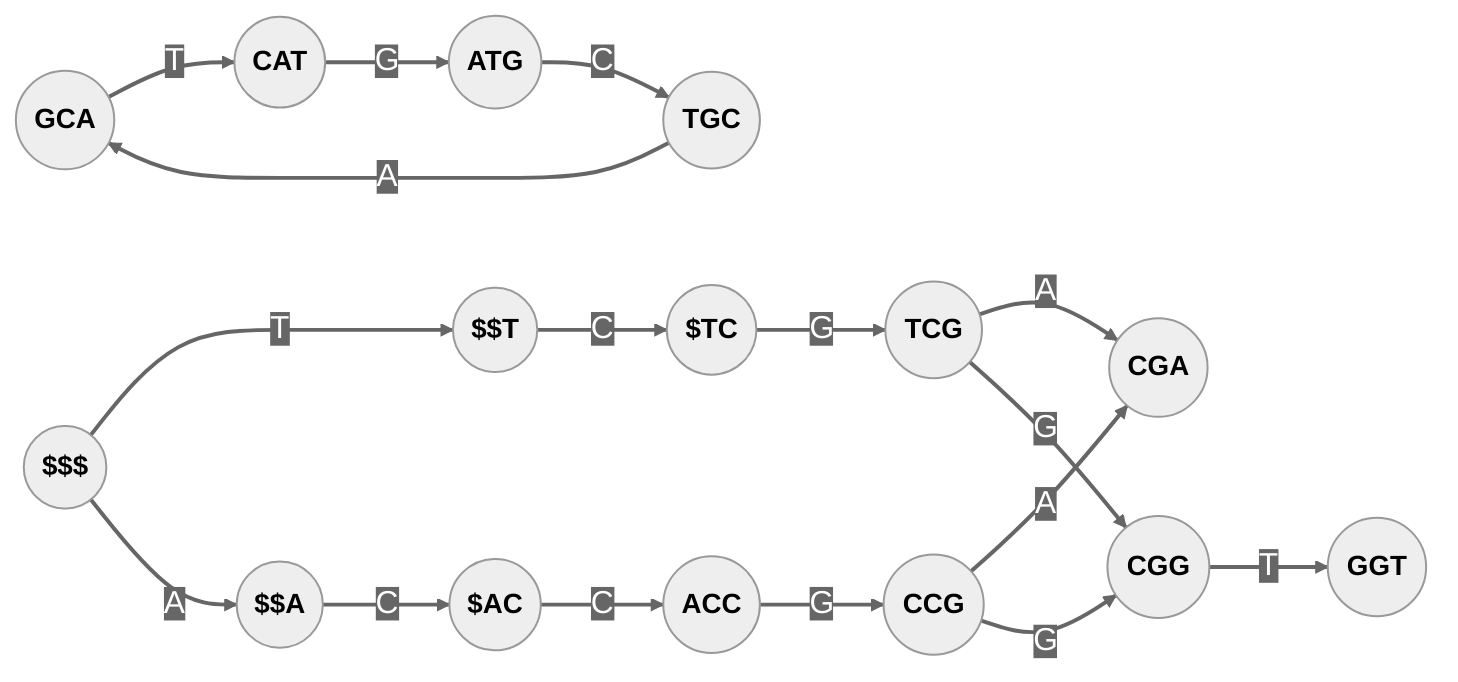
\includegraphics[width=\textwidth]{images/FastaqToDbgWithDollars.png}
  \caption{The altered DBG from Figure~\ref{fig:FastaqToDbg} where extra $\$$ nodes are added to existing nodes with no incoming edges with extra \$-symbols.}\label{fig:FastaqToDbgWithDollars}
\end{figure}
